\section{Tilt switch}
\begin{figure}[H]
    \centering
    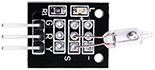
\includegraphics[angle=0, keepaspectratio=true, scale=1, width=200px, height=200px]{images/tilt.jpg}
    %\caption{Caption}
\end{figure}
\subsection*{Description}
This module contains a small amount of conductive liquid in a tube. When the liquid moves to one end of the tube the output voltage is either pulled high or low, and vice versa for the other end. This allows us to monitor if the module is upside down or not.
\subsection*{Pin mapping}
This pin mapping corresponds to the pins from left to right with the module pins facing towards you.
\begin{table}[H]
    \centering
    \begin{tabular}{|c|c|c|c|c|}
    \hline
    Index &Label &Type &Name &Description\\ \hline
    0 &- &Ground &GND &\\ \hline
    1 & &Source voltage &$V+$ &Module source voltage ($5V$)\\ \hline
    2 &S &Digital output &D0 &\\ \hline
    \end{tabular}
    %\caption{Caption}
    %\label{tab:my_label}
\end{table}
\subsection*{Operation}
When the module is upright (not upside down) the voltage of the digital output pin D0 is low. When the module is upside down the voltage of D0 will be set to high.
\subsection*{Code}
Refer to listing \ref{python_tiltswitch}.
%\lstinputlisting[caption=test]{laser.py}